%%%%% FORMAT THE PAPER %%%%%%%%%%%%%%%%%%%%%%%%%%%%%%%%%%%%%%%%%%%%%%%%%%%%%%%%%

%\documentclass[final, 12pt]{thesis}  % this looks okay. (AAK, 8/2/08)
%\documentclass[final,10pt,oneside]{thesis}
%\documentclass[compact,10pt]{thesis}  % this looks like shit. (AAK, 8/2/08)
%\documentclass[compact,12pt,twoside]{thesis}  % this looks like shit. (AAK, 8/2/08)
\documentclass[final,12pt,oneside]{thesis}
%\documentclass[final,12pt,twoside]{thesis}
%\documentclass[draft,12pt]{thesis}
        % Curly brackets: Specify the "thesis" class file (thesis.cls).
        %   It assumes the existence of a few other style (*.sty) files.
        %   See the thesis.cls file for details.
        % Square brackets, specify the options you want to use.
        %   Allowed options are 10pt, 11pt, 12pt,
        %   oneside, twoside, draft, compact, and final.
        %   See the "thesis.cls" file for descriptions.

%%%%% INCLUDE PACKAGES %%%%%%%%%%%%%%%%%%%%%%%%%%%%%%%%%%%%%%%%%%%%%%%%%%%%%%%%%

% NOTE: If you want your figure captions, table captions, and bibliography
% items single-spaced (this is permissible for UW theses!), you can use
% the "\fixspacing" command in each of these environments.  This command
% will choose the appropriate spacing, whether you use the "final" or
% "draft" modes.  See the "thesis.cls" class file for details.
% CLARIFICATION: The \fixspacing command has to go inside EACH of your
%     \tablenotetext blocks to be effective

%\usepackage[showframe,pass]{geometry} % Shows borders on the page.
\usepackage{graphicx}
\usepackage{amssymb}		% AMS symbols
%\usepackage{threeparttable}
\usepackage{latexsym}
\usepackage{natbib}
\usepackage{chapterbib}
\usepackage{xspace}
\usepackage{amsmath,amssymb}		% package to get fancy math stuff
\usepackage[usenames,dvipsnames]{color}
%\usepackage[draft]{hyperref}
\usepackage{hyperref}
\hypersetup{
    pdftex,
    pdftitle={Your title},
    pdfauthor={Your Name}
}
%\usepackage{tabularx}
%\usepackage{subfig}
%\usepackage[FIGTOPCAP]{subfigure}
%\usepackage{upgreek}
%\usepackage{multirow}
%\usepackage{longtable}
%\usepackage{tabularx}
%\usepackage{siunitx}

%\usepackage{etoolbox}
%\appto\TPTnoteSettings{\footnotesize}
%\usepackage{lscape}		% package for landscape-style pages
% You can use this to create a landscape table in a \begin{landscape}--
% \end{landscape} environment.  Note that the rotated table will probably *not*
% show up in Xdvi, but *will* show up in the PostScript version (e.g., can be
% seen with gv).

%\usepackage{nomencl}	% For creating lists of abbreviations and symbols

%\makenomenclature
%\makeindex

%\makeatletter
%\g@addto@macro\TPT@defaults{\footnotesize}
%\makeatother

\citestyle{aa}

%\newcommand{\red}[1]{{\color{red} #1}}
%\newcommand{\green}[1]{{\color{green} #1}}
%\newcommand{\blue}[1]{{\color{blue} #1}}

\newcommand{\degrees}{\ensuremath{^{\circ}}}
\newcommand{\NII}{[\ion{N}{ii}]}
\newcommand{\SII}{[\ion{S}{ii}]}
\newcommand{\Halpha}{H\ensuremath{\alpha}}
\newcommand{\Hbeta}{H\ensuremath{\beta}}
\newcommand{\Lyalpha}{Ly\ensuremath{\alpha}}

\newcommand{\kms}{km~s$^{-1}$}
\newcommand{\OonH}{\ensuremath{12+\log(\mathrm{O/H})}}

\newcommand{\f}{\emph{f}/}

\newcommand{\GP}{$\nabla$Pak\xspace}
\newcommand{\Ha}{\ensuremath{\mathrm{H}\alpha}\xspace}
\newcommand{\HB}{\ensuremath{\mathrm{H}\beta}\xspace}
\newcommand{\Hd}{\ensuremath{\mathrm{H}\delta}\xspace}
\newcommand{\Hg}{\ensuremath{\mathrm{H}\gamma}\xspace}
\newcommand{\He}{\ensuremath{\mathrm{H}\epsilon}\xspace}
\newcommand{\Zsol}{\ensuremath{\mathrm{Z}_{\odot}}\xspace}
\newcommand{\tauV}{\ensuremath{\tau_{\mathrm{V,cont}}}\xspace}
\newcommand{\tauVB}{\ensuremath{\tau_{\mathrm{V,Balmer}}}\xspace}
\newcommand{\val}[2]{\ensuremath{#1~\mathrm{#2} \xspace}}
\newcommand{\sol}[1]{\ensuremath{#1_{\odot} \xspace}}
\newcommand{\mum}{\ensuremath{~\mu\mathrm{m}}}
\newcommand{\fn}{$f$/\#\xspace}
\newcommand{\fratio}{$f$-ratio\xspace}
\newcommand{\filtB}{\val{440}{nm}\xspace}
\newcommand{\filtI}{\val{790}{nm}\xspace}
\newcommand{\filty}{\val{551}{nm}\xspace}
%\newcommand{\arcsec}{\mbox{$^{\prime\prime}$}}
%% \newcommand{\farcs}{\mbox{$\!\!^{\prime\prime}$}}
%% \newcommand{\arcmin}{\mbox{$^{\prime}$}}
%\newcommand{\f}{\emph{f}/}
	% Read in list of user-defined LaTeX commands

%%%%% SELECTIVE COMPILATION %%%%%%%%%%%%%%%%%%%%%%%%%%%%%%%%%%%%%%%%%%%%%%%%%%%%

% Uncomment to prevent the creation of new *.toc *.lot, and *.lof
%   files.  Do this if you need to edit these files for the final
%   version of the paper.  For example, if you have multi-page
%   figures or tables but you want the lists of figures & tables
%   to have only one line for these, you will need to delete the
%   extra lines in the *.lof and *.lot files and re-run LaTeX.
%\nofiles

% Use \includeonly{} if you are just working on one \include{}'d
% section.  This prevents LaTeX from re-processing the unneeded
% chapters, but preserves references and page/fig/table numbers.
% Try it.  You'll like it.
%\includeonly{Abstract}
%\includeonly{Introduction/Introduction}
%\includeonly{Chap2/chap2}
%\includeonly{Conclusion/Conclusion}

%%%%% BEGIN THE DOCUMENT %%%%%%%%%%%%%%%%%%%%%%%%%%%%%%%%%%%%%%%%%%%%%%%%%%%%%%%

\begin{document}        % BEGIN THE DOCUMENT TEXT

% Force some caption formatting
%\captionsetup[table]{justification=centering,font=rm,labelsep=none}
%\captionsetup[figure]{font=rm,labelsep=none}

%%%%% TITLE PAGE %%%%%%%%%%%%%%%%%%%%%%%%%%%%%%%%%%%%%%%%%%%%%%%%%%%%%%%%%%%%%%%
\title{My Thesis}

\author{Your Name}
\year{1955}

% These two aren't really needed except for the UMI abstract
\adviser{Dr.\ Awesome Advisor}
\adviserrank{Associate Professor}

\oralexamdate{5 November 1955}
\committeeone{Member One, Associate Professor, Astronomy}
\committeetwo{Member Two, Professor, Astronomy}
\committeethree{Member Three, Assistant Professor, Astronomy}
\committeefour{Member Four, Professor, Astronomy}
\committeefive{Member Five, Professor, Physics}

\ttlpage                % This command produces the title page.  Nifty!
%\cpypage                % This produces the copyright page.  Also nifty!
                        % Reminder: it costs money to register copyright
                        % (but you *have it* without doing anything!)

\cleardoublepage

%%%%% FRONT MATTER: ABSTRACT, DEDICATION, ACKNOWLEDGMENTS, CONTENTS %%%%%%%%%%%%

\frontmatter            % Choose roman-type numbers; reset page numbers to 1.

\pagestyle{thesis}      % Set the page style to "thesis"
                        %   (page numbers at the top right)

%% \chapter*{Abstract}
\addcontentsline{toc}{section}{Abstract}

Studies of the Milky Way show that the vertical velocity dispersion of
stars in the disk tends to increase with age, but it is not clear how
this ``heating'' ties into the formation of the observed Milky Way
structure, and disk galaxies in general. In this thesis I present a
study of stellar populations in NGC 891 that adds information to our
information on the structure of galaxies outside the Milky Way. 

This study was enabled by the construction of HexPak/\GP, two fiber
integral field units that together form the worlds first dual-head,
multi-pitch fiber instrument. Specifically, the unique design of \GP
allowed for the rapid collection of high quality data over a large
range in surface brightness and at a high filling factor. When
designing HexPak/\GP I investigated sources of fiber focal ratio
degredation and found that surface scattering likely plays a large
role in the degredation of light emitted by fiber optics.

Using \GP I find that the overall picture of disk heating in NGC 891
is remarkably similar to trends measured in the Milky Way; the
presence of young populations is abruptly cut off at \asim 1 scale
height. Furthermore I find that populations generally get younger
farther from the center of NGC 891, which is perhaps the signature of
an inside-out formation scenario.

Finally, I identify three distinct features in NGC 891: (i) a primary
disk(s) that exhibits the same general trends seen in the Milky Way,
(ii) a flared extension of this disk at large radii ($>
\val{8}{kpc}$), and (iii) a super metal-rich sequence of stars at
large radii and heights that is difficult to explain, but is perhaps
the remnant of some very early flare.
      % *.tex file for abstract
%% \cleardoublepage

%% %\include{sponsor}       % *.tex file for "sponsorship" page

%% %\include{Dedication}      % *.tex file for dedication
%% %\cleardoublepage

%% \chapter*{Acknowledgments}
\addcontentsline{toc}{section}{Acknowledgments}

Humans cannot live on work alone, and without a good outlet for
frustration and pent up energy I would probably be on a lot more
governmental watchlists. Credit must first be given to Matt Bershady;
without your expert guidance and truly shocking (dangerous?)
willingness to listen to what I had to say none of this would have
been possible. You always pushed me just past my comfort zone and told
me \emph{what} to do, not \emph{how} to do it (until I did it wrong a
few times). The past six years rank extremely high in the epochs of my
development as a legit scientist, and I expect them to remain there
for a long time.

Beneath the Ivory Tower, in the beautiful slums of grad school, the
passage of time has been eased immeasurably by many of my fellow
travelers. To Andrew and Corey, thanks for being great research
partners. To Danielle and Britt, your feline obsession did little to
temper the pleasure of spending my first 2 years in your company. To
the Atom: Anna, Chris, Jenna, and John; thanks for giving me a couch
that I could use to get away from the cat talk. That and a lot of
snacks and scientific insight. Special mention is gladly given to
Jenna, who unwittingly accompanied me through the last 10 years. From
throwing lemons at East to biking to Michael's; it's been real. To
Diego, DK, Julie, and Max, the Young Blood that keeps me energized,
thanks for reducing the thickness of my jade layer with your youthful
enthusiasm and adorable 1st year problems. Me g\`usta. To Claire and
Elijah; sometimes a trip down the hall was all I needed and you
tolerated my interruptions with grace and good humor.

It would be impossible understate the importance of my family to my
apparent success. Unwavering support, unconditional love, and copious
amounts of Night Train are all crucial ingredients in the foundation
of this work.

To Mary, you have been with me through the thickest and the thinnest
and for that I will be forever grateful. You drive me to be the person
you think I am and are always willing to forgive my failings.

To Anna, the best student I ever had, your steadfast determination to
move forward despite fear and uncertainty is a continuing inspiration.

Thank you so much to The Begowatts, members past and present; you gave
me an outlet for the squishier parts of my brain and something to do
when I just wanted to hit something.

A very special thanks to the City Bar for being a refuge from the
storm. Kevin and MJ, you are the best bartenders I've ever had the
privilege to buy beer from; thanks for providing a welcoming
environment and slinging some wicked suds.

And finally, without music to dull the baser parts of my psyche none
of this would have happened. In the end recognition must be given to
The Boss for reminding me that being earnest can be cool, The Band
for so much joy (and especially ``Ophelia''),
NRW\footnote{\url{https://www.youtube.com/channel/UCAZ77vdqYbuGbCAWB62WbqQ}}
for a great background, and B{\"O}C for being with me from the
beginning.
        % *.tex file for acknowledgements
%% \cleardoublepage

%\include{quotes}        % *.tex file for quotations
%\clearpage

\setcounter{tocdepth}{3}
\tableofcontents        % *.toc file with table of contents
\cleardoublepage

%% \listoftables           % *.lot file with list of tables
%% \clearpage

%% \listoffigures          % *.lof file with list of figures
%% \cleardoublepage

     % Note that the \listoftables does not play well with the
     % deluxetable environment.  You will probably have to do some
     % hand-tweaking of the master.lot file if you have multi-page
     % tables.

%\renewcommand{\nomlabel}[1]{\hfil #1\hfil}	% Center symbols in list
%\renewcommand{\nomname}{List of Abbreviations and Symbols}

%\clearpage
%\addcontentsline{toc}{section}{List of Abbreviations and Symbols} % add contents line; does not use default given by nomencl package also usually puts in the wrong page number, change it in master.toc

%{\fixspacing \small
%\printnomenclature[1in]	% *.nls file with list of symbols
%}

%\cleardoublepage


%%%%% MAIN TEXT OF THE THESIS %%%%%%%%%%%%%%%%%%%%%%%%%%%%%%%%%%%%%%%%%%%%%%%%%%
%manually widening the vertical spacing between text
%\renewcommand{\baselinestretch}{1.4}

\mainmatter

% I don't have any tables, so table column separation is not of concern.
%\setlength{\tabcolsep}{0.035in}

\chapter[Introduction]{Introduction}
\label{chap:intro}

% Leave space between title and quote or publication note.  This has often been
% 10cm for a quote and 8 cm for a reference, but this is really up to you.
%\vspace{8cm}

%\vfil\eject\clearpage
\clearpage It has long been known that stars in the solar neighborhood
have vertical scale-heights and velocity dispersions that increase
with age \citep[e.g.,][]{Wielen74}. This phenomenon is referred to as
``disk heating'', and the origin of this heating process has never
been settled. Unfortunately, our empirical constraints on disk heating
come only from the solar cylinder in the Milky Way and a few crude
measurements of low-mass edge-on spirals close enough for HST
star-counts \citep{Seth05a}. This scant data is insufficient to
resolve several outstanding questions: How does the heating rate
evolve with time and radius?  Why does disk heating in the Milky Way
appear to saturate after about 5 Gyr?  What, then, gives rise to the
thick disk?  And is heating in the Milky Way representative of disk
galaxies in general? Answers to these questions have critical
implications for our picture of disk evolution, all the more poignant
given recent observational claims that high-redshift ionized gas disks
are dynamically hot, clumpy, and thick \citep{Forster-Schreiber09} and
models \citep{Bird13} that predict the formation of observed current
disk structure from these high-redshift disks.

Clearly more data is needed, and the rise of resolved spectroscopic
surveys of external galaxies (e.g., MaNGA, SAMI, CALIFA) will offer a
new window into the distribution of stellar populations outside the
Milky Way. However, these surveys lack the spatial resolution
necessary to make detailed comparisons to the substructures seen in
the Milky Way and it is crucial to complement their broad scope with
focused measurements of nearby galaxies. NGC 891 offers an attractive
target for such a study; it is nearby, almost perfectly edge-on, and
is thought to be a good Milky Way analog. In this thesis I present a
study of stellar populations in NGC 891, specifically where these
populations fall in a six dimensional space containing three position
dimensions along with age, metallicity, and extinction.

The rest of this chapter is organized as follows: in
\S\ref{intro:sec:MW} I review the picture of disk formation as
revealed locally in the Milky Way; in \S\ref{intro:sec:SSP} I discuss
the details of the methods (namely full-spectral fitting) that will be
used to measure populations in NGC 891; and in \S\ref{intro:sec:fiber}
I give a brief overview of fiber integral field units (IFU) and lay
the groundwork for the introduction of HexPak/\GP; the world's first
dual-head, variable-pitch IFU.

\section{Stellar Populations in the Milky Way}
\label{intro:sec:MW}
\begin{figure}
  \centering
  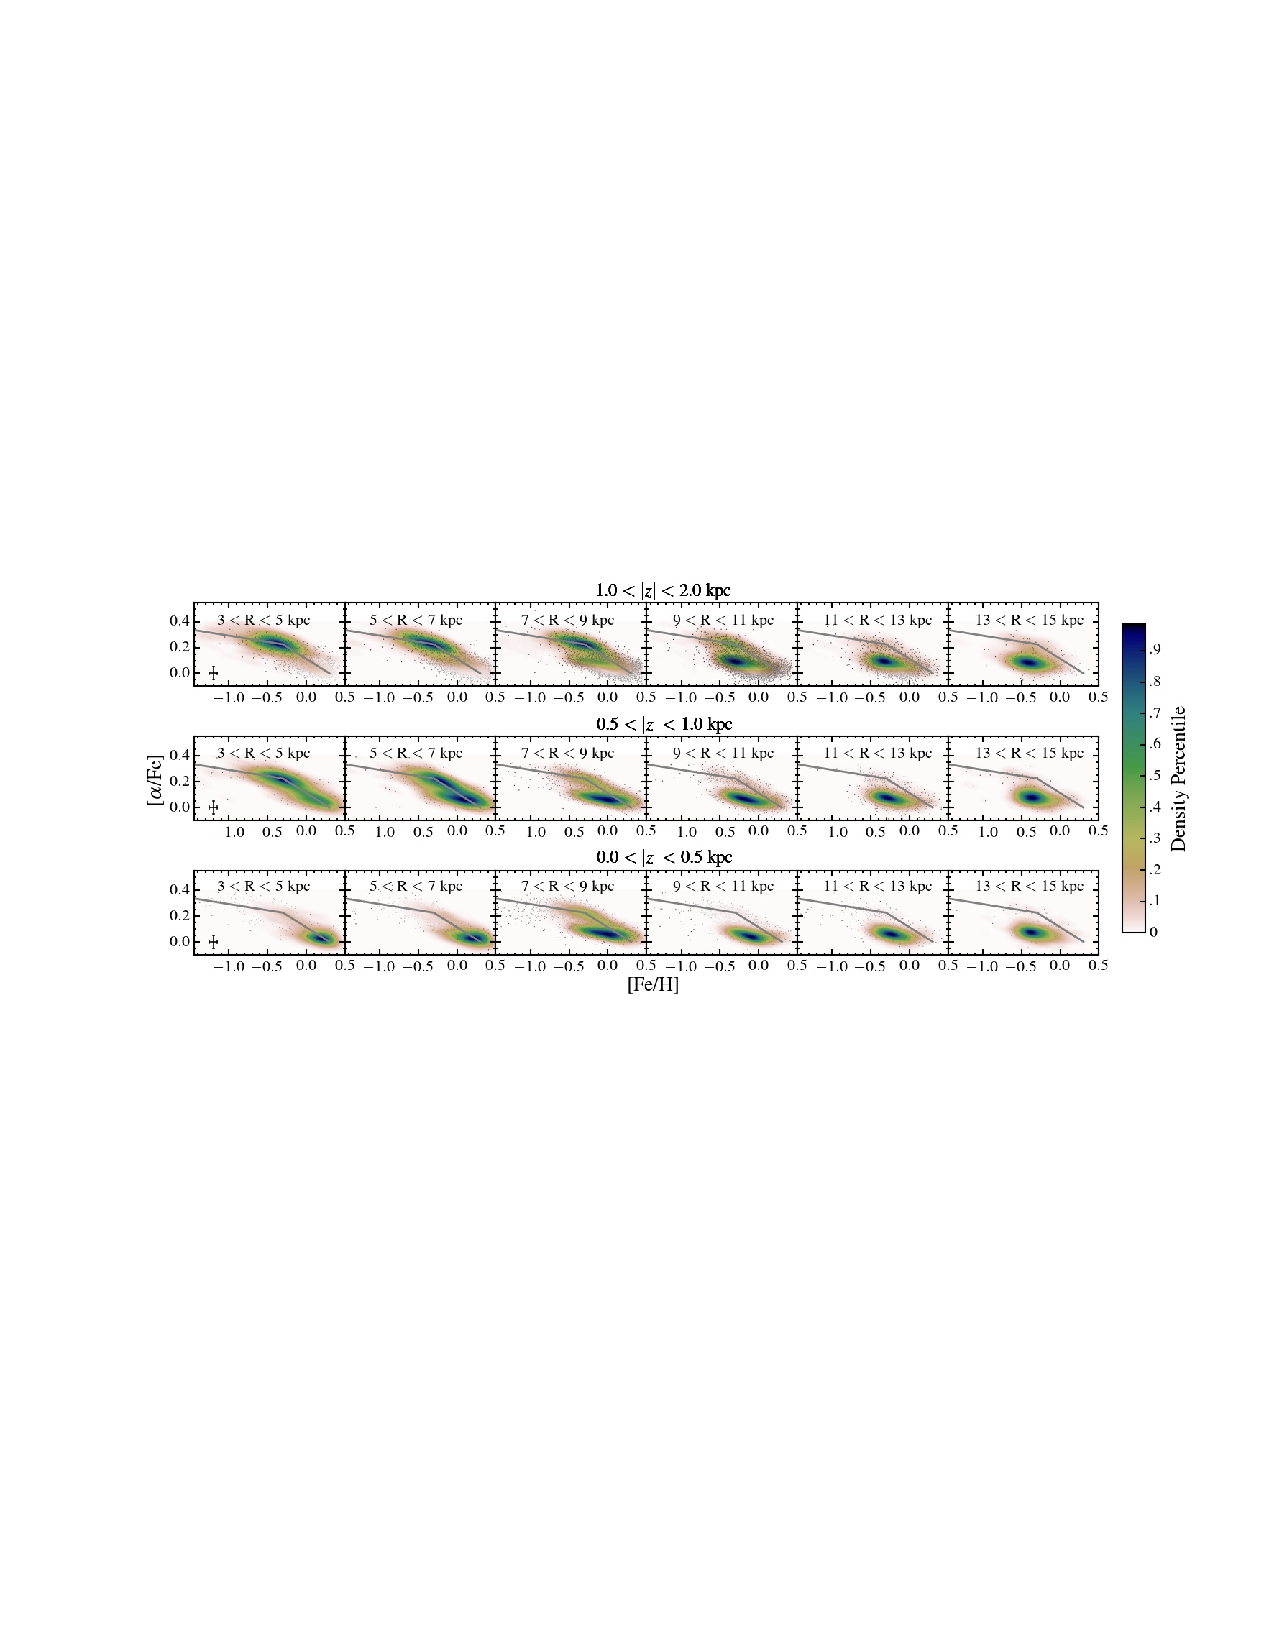
\includegraphics[width=\textwidth]{Introduction/figs/hayden_15.pdf}
  \caption[Metallicity and abundance of solar cylinder stars as a
  function of radius and
  height]{\fixspacing\label{intro:fig:hayden}The distribution of stars
    near the Sun in the [$\alpha$/Fe] vs. [Fe/H] plane, presented in a
    grid of radius and height. From \citet{Hayden15}.}
\end{figure}

By the middle of the last century it was well established that the
scale-heights and velocity dispersions of stars in the solar
neighborhood increase with age \citep[see][for a summary of this early
work, particularly the chapters contributed by Elvius and
Delhaye]{Blaauw65}. The seminal work by \citet{Roman50} demonstrated
that the disk kinematics also depended on metallicity.  Today these
patterns are known in the literature on Galactic archaeology as
age-velocity-metallicity (abundance) relations \citep[AVM$\alpha$-R;
e.g.,][]{Aumer09,Minchev14}. Observational advances continued for the
solar neighborhood \citep[e.g.,][]{Edvardsson93, Dehnen98,
  Nordstrom04}, and by the beginning of this century the complexity of
these relations had been mapped throughout much of Milky Way (MW) by
wide-field spectroscopic surveys (e.g., RAVE, \citealt{steinmetz06a};
BRAVA, \citealt{howard08a}, SEGUE, \citealt{yanny09a}, LAMOST,
\citealt{zhao12a} GALAH, \citealt{desilva15a},
Gaia-ESO,\citealt{gilmore12a}; and APOGEE-1 and -2,
\citealt{Majewski15}). The radial gradients in these relations are
beautifully shown in Figure \ref{intro:fig:hayden} (from
\citet{Hayden15}), illustrating the usefulness of both metallicity and
abundance as well-known, complementary chemical-evolutionary
tracers. Despite a century of remarkable progress, two broad but
intertwined questions remain: (i) What are the astrophysical processes
(i.e., the chemo-dynamical explanation) leading to the observed
relations?; and (ii) are these patterns generic for spiral disks or
specific to the Milky Way?

\begin{figure}
  \centering
  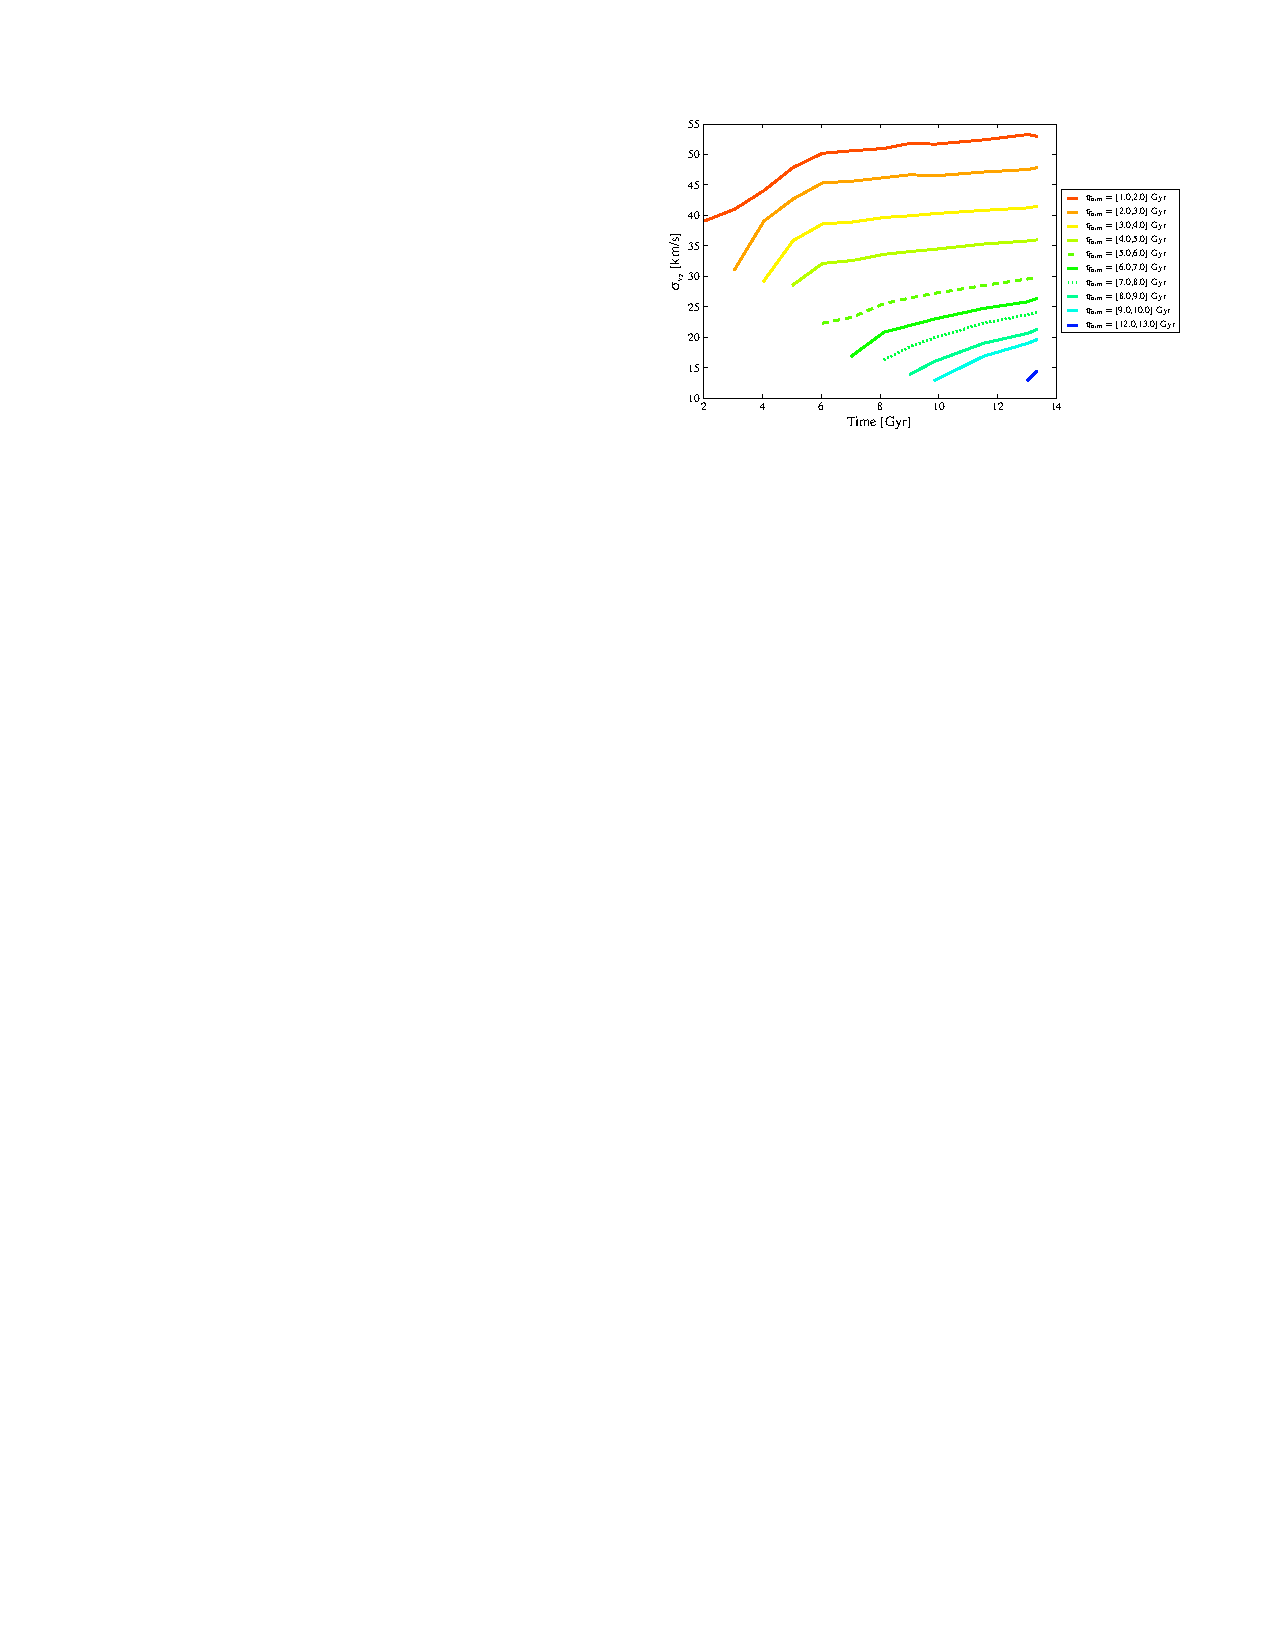
\includegraphics[width=0.8\textwidth]{Introduction/figs/bird_13.pdf}
  \caption[Dynamical settling in a Milky-Way-like galaxy
  model]{\fixspacing\label{intro:fig:bird}Vertical velocity dispersion
    of stellar populations with different formation ages as a function
    of time. These models are based on hydrodynamical simulations of a
    Milky-Way-like disk galaxy. From \citet{Bird13}}
\end{figure}

Setting aside chemical evolution for simplicity, there has been a
long-standing debate about the origin of the vertical stratification
of disk stars in phase-space as a function of age. This stratification
is known as the the age-velocity relation, or AV-R. Historically the
argument has been in the context of dynamical heating from two-body
scattering \citep{Spitzer51}, but the source of this scattering has
been debated \citep[e.g., giant molecular clouds, transient spiral
structure, or dwarf satellite
galaxies][]{Spitzer51,Spitzer53,Wielen77,Quinn93,Binney00}, and none
have proven satisfactory to explain the MW's thick disk.  This
framework has been salvaged but also up-ended by relatively recent
evidence for the increasing turbulence (and presumably thickness) of
ionized gas in disks at higher redshifts
\citep{Weiner06,Forster-Schreiber09,Wisnioski15}. It seems plausible
that early phases of disk formation involved gas cooling, leaving
behind an old, thick-disk stellar component
\citep{Brook04,Bournaud09}. However, thinner relic layers would also
emerge as time progressed \citep{Bird13}, depending critically on the
cooling time-scale for the gas in the presence of star-formation, AGN
feedback, and accretion. Figure \ref{intro:fig:bird} shows an example
of this theory; vertical velocity dispersion does slightly increase as
stars age (i.e. ``heating''), but the dominant trend is that more
recently formed populations are dynamically cooler. Ironically, this
``settling'' of the stellar disk is not unlike the predictions of
monolithic collapse from \citet{ELS}, albeit now consistent in the
context of bottom-up, or hierarchical structure formation as seen in
recent simulations \citep[e.g.,][]{Bird13,Martig14a}.  It is no longer
clear if, loosely speaking, disks ``heat'' or ``cool'' to form the the
vertical stratification of disk stars in phase-space, and likely both
modes play a role at late and early times, respectively. For this
reason we refer instead to ``dynamical stratification'' as a
phenomenon that captures both general physical processes.

The recent simulations noted above show there is a rich history of
radial and vertical build up of stellar populations that involves an
interplay between the cooling of the gas, the impact of mergers and
accretion, and, at late times, the classical heating processes noted
above.  This richness suggests the possibility for a diversity of
astrophysical paths in disk formation that could lead to significantly
different structure in galaxies, exhibited in their
AVM$\alpha$-Rs. Hence, the broader question of whether the MW is
representative of the external disk galaxy population becomes salient.

%% Maybe move to previous section
Little is known about the dynamical stratification rates for stars in
spiral galaxies outside the Milky Way, but recent studies of stellar
populations and dynamical stratification in low-mass spiral galaxies
\citep{Seth05a,Bernard15} have shown dramatic differences in the
age-metallicty and age-velocity dispersion relations when compared to
the Milky Way. Recent measurements of the stellar velocity dispersions
in M31 \citep{Dorman15} show that there are gradients in dispersion
with age and metallicity, but with amplitudes and time-scales that are
larger than in the MW. Differences in velocity dispersion amplitudes
may reflect a more massive or thinner M31 disk, but possibly also a
different dynamical history -- for gas settling or stellar dynamical
heating. Clearly more data on the stellar properties of external
galaxies is needed. The above studies serve as a gold standard since
they are based on studies of resolved stellar populations. Because
there are no massive spiral galaxies outside of the Local Group for
which we can resolve stellar populations at surface-densities high
enough to probe most of the disk, it is imperative to undertake
studies based on integrated starlight.

\section{Deriving Population Properties with Full Spectrum Fitting}
\label{intro:sec:SSP}
\begin{figure}
  \centering
  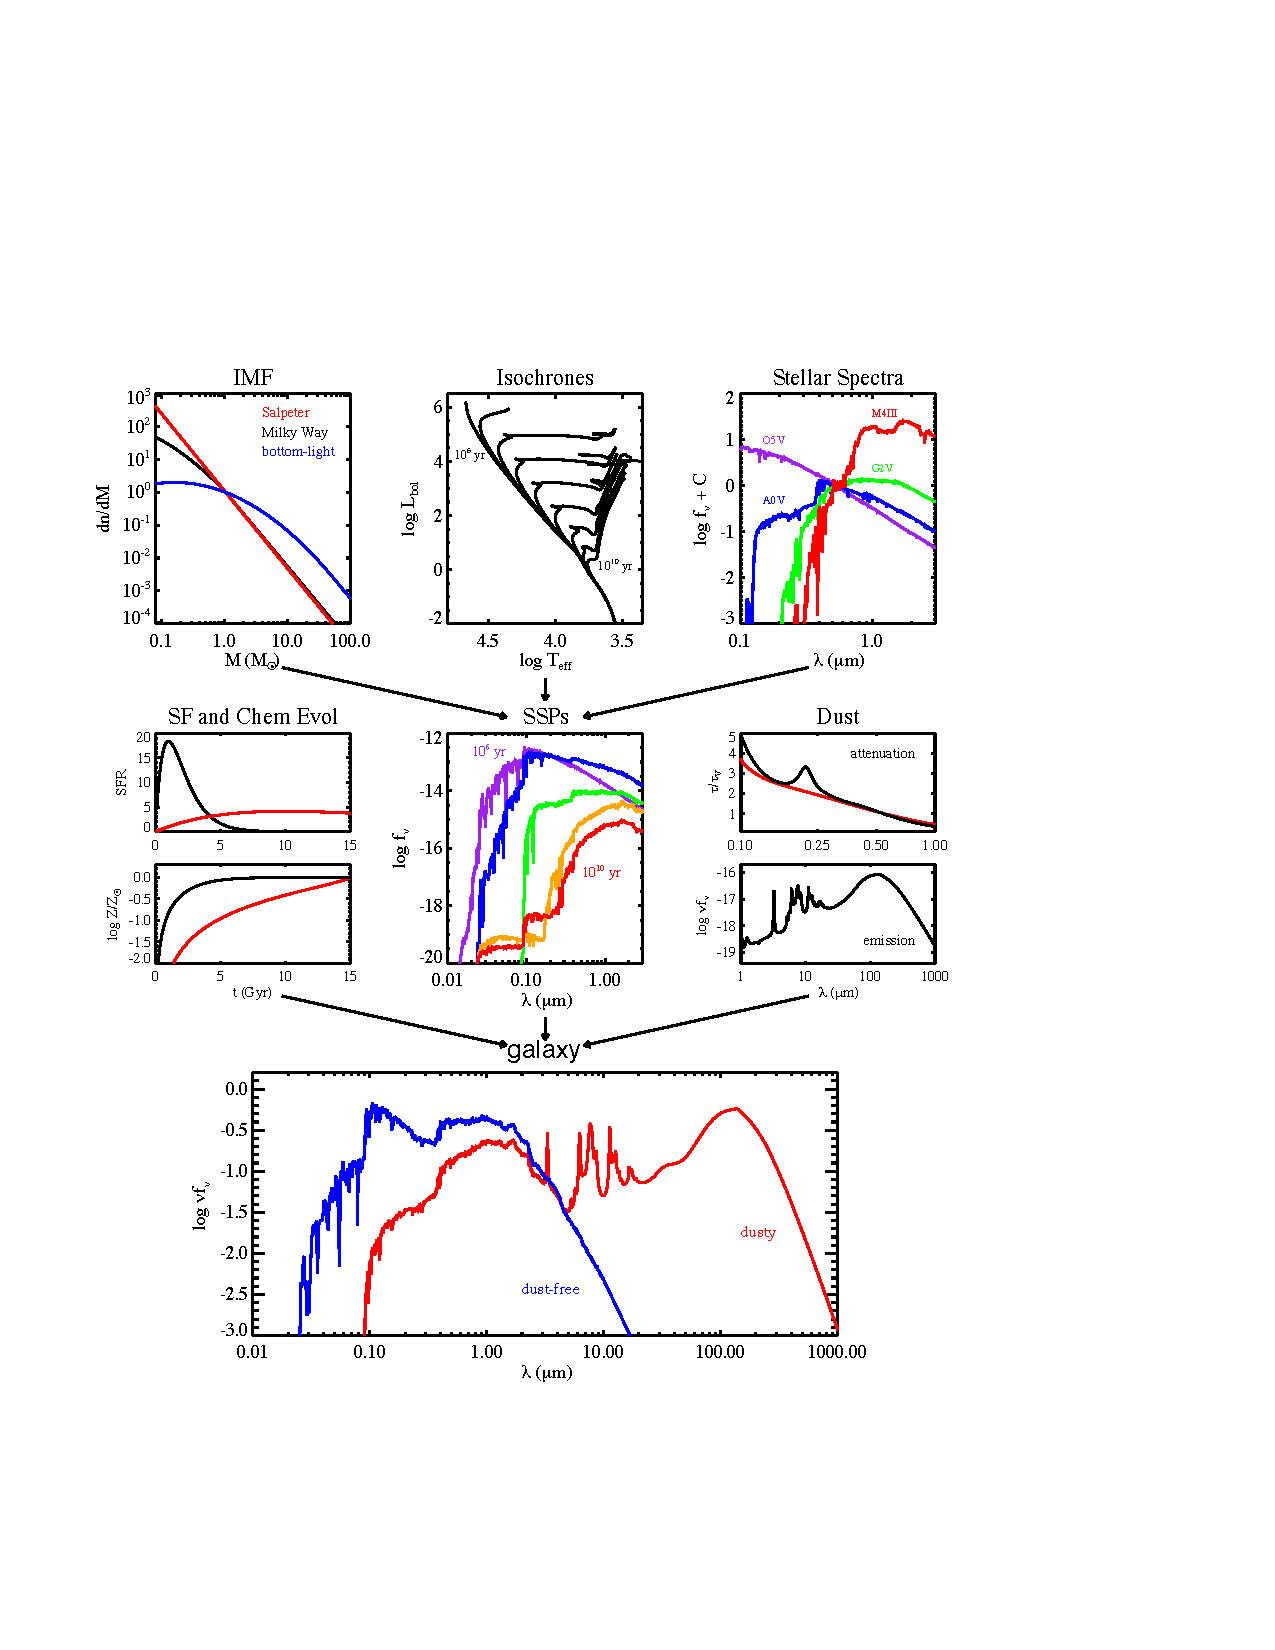
\includegraphics[width=0.8\textwidth]{Introduction/figs/conroy_13.pdf}
  \caption[Schematic of full spectrum
  fitting]{\fixspacing\label{intro:fig:conroy}The important components
    of full spectrum fitting. An initial mass function (IMF),
    isochrones, and spectra are combined to construct individual
    SSPs. Multiple SSPs are then combined, with and assumed star
    formation history and dust properties, to form a model
    galaxy. From \citet{Conroy13}.}
\end{figure}

In this work we employ full-spectral fitting to measure age,
metallicity, and extinction as a function of radius and height in NGC
891. The idea of modeling integrated starlight (i.e., a spectrum) to
measure galaxies properties has a long history since \citet{Spinrad71}
first manually mixed stars together, and modern techniques employ a
variety of sophisticated methods to extract the maximum about of data
from each wavelength. Regardless of the specific method, all attempts
at full-spectrum fitting require the same basic ingredients: (i) a
library of stellar spectra, whether empirical or synthetic, (ii) a set
of isochrones that encapsulate how stars evolve with time, and (iii)
an initial mass function (IMF). With these three components
Astronomers can construct simple stellar populations (SSPs); a set of
stars of the same age and same metallicity/abundance with a mass
distribution determined by the IMF. To simulate an entire galaxy
multiple SSPs of different ages and metallicities are combine together
to produce a complex stellar population (CSP), which requires assuming
both a star formation history (SFH) and the distribution/properties of
dust in the galaxy. An excellent discussion of this process can be
found in \citet[and his diagram shown in Figure
  \ref{intro:fig:conroy}]{Conroy13}.

Within the general picture painted above there exists a wide range of
options and data. It is common for SSP libraries to be constructed
with the Padova isochrones \citep{Bertelli94, Girardi00, Marigo08}
because these models cover the widest range of stellar age and
chemical compositions, but other models are often used for their focus
on specific epochs of stellar evolution. For example high-mass stars
(Geneva \citep{Schaller92,Meynet00}), low-mass stars ($Y^2$
\citep{Yi01,Yi03}, or Dartmouth \citep{Dotter08}), and even very
low-mass stars (Lyon \citep{Chabrier97,Baraffe98}). In this work we
use exclusively the Padova isochrones because our observations, by
their very nature, are light-weighted and therefore the specific
details of low mass stars are relatively unimportant.

The choice of IMF can also affect the final modeled galaxy
spectrum. The canonical IMF of \citet{Salpeter55} was based on
observations of the Solar Cylinder in the Milky Way, and there is so
far little evidence that the IMF is appreciably different elsewhere in
the Universe \citep{Bastian10}. More recent observations have refined
the specific form of the IMF \citep{Kroupa01, Chabrier03}, but the
general picture remains the same. We use the IMF of \citet{Chabrier03}
because it is physically motivated and provides a good fit to low-mass
and brown dwarf star counts in the Milky Way
\citep{Bruzual03,Chabrier01,Chabrier03}.

Finally, the construction of SSPs depends on the stellar library
used. In this work we consider only empirical stellar libraries, and
more specifically the STELIB \citep{LeBorgne03} and MILES
\citep{Sanchez-Blazquez06} libraries. The main strength of empirical
libraries is that they get the chemistry right by default, as indeed
they must. The cost of this accuracy, however, is a very limit
sampling of the entire parameter space of stellar evolution. For
example, as is discussed in \S\ref{891_2:sec:ma11}, the MILES library
very coarsely samples the metallicty/age plane and doesn't have any
spectra for ages below \val{6.5}{Myr}. 
% Ultimately, we use the STELIB
% library because it more finely samples stars of different ages, but
% warn that it still lacks a detailed view of how spectra change with
% metallicity.
As discussed in \S\ref{891_2:sec:SSP_sets} we ultimately use the SSPs
of \citet{Bruzual03}, which are constructed with the Padova
isochrones, Chabrier IMF, and STELIB library. We note, however, that
over the wavelength range we consider ($\val{3800}{\AA}
\leq\lambda\leq \val{6800}{\AA}$) the differences in spectral shape
caused by different assumptions/models are minimal.

More directly relevant to our work is the assumption about the SFH
that is used to construct galaxies (CSPs) from SSPs. A common choice
for SFH is the so called $\tau$-model where the star formation rate
(SFR) follows an exponential function with a single scale parameter,
$\tau_\mathrm{SF}$. This analytic form is based on closed-box models
where the SFR depends linearly on gas density \citep{Schmidt59} and
offers an attractive, one parameter, parameterization of the SFH. In
this work we chose to use a non-parametric SFH (as discussed in
\S\ref{891_2:sec:SSP_method}) which allows us to reduce the
systematics in our results that arise from forcing an analytic form of
the SFR (systematics are not completely eliminated, however, as
discussed in \S\ref{891_2:sec:sys_err}). Using this method results in
a much larger set of free parameters and puts more strain on the
fitting code, but our data have high enough signal to noise
(\val{\asim 30}{px^{-1}}) to make it a viable option.

Once model galaxies are constructed there are a multitude of methods
available to fit them to our data, for example those of
\citep{Cappellari04, Tojeiro07,Chen12, CidFernandes05, Ocvirk06,
  Wilkinson15, Sanchez16}. Regardless of the method used these fits
face the same common issues; namely how to deal with known
degeneracies between age, metallicity, and extinction
\citep{Oconnel76,Aaronson78,Worthey94,dePaz02}. In some methods the
extinction degeneracy can be mitigated by removing the overall
continuum from both the data and models before fitting
\citep[e.g.,][]{Ocvirk06,Wilkinson15} and then recovering an
extinction estimate either by measurements of gas emission (i.e., the
Balmer decrement) or separate analysis of the ``best fit'' galaxy
spectrum. Metallicity and age are more closely entwined and the
degeneracy between them more difficult to break. In this work we
attempt to quantify the uncertainties that arise from similarities
between SSPs that are degenerate with age and metallicity (see
\S\ref{sec:fit_err}), but note that we have not addressed systematic
uncertainties that may arise from our choice of model SSPs.

\section{A Fiber Optic Primer}
\label{intro:sec:fiber}
The use of fused silica optical fibers for astronomical observations
was first suggest by \citet{Angel77}, and in the intervening decades
their importance and usefulness to Astronomy has only increased. The
astronomical benefits of fiber optics are essentially two fold:
Firstly, they allow instruments to be decoupled from the telescope
focal plane, which enables the construction of very large and
sensitive spectrographs that are free from the unstable environmental
conditions often found on the observing floor. Secondly, they can be
easily placed at an arbitrary position on the sky while maintaining a
consistent spectrograph input.

A class of fiber optic instruments called integral field units (IFUs)
make great use of this second point. IFUs are a collection of fibers
that are placed in some two-dimensional configuration on the sky and
therefore produce data that exist in three dimensions (two spatial and
one spectral). Some IFUs are designed to efficiently measure the
spectra of a large field of stars, for example HYDRA {\bf REF? Can't
  find it!}, and can have the location of their fibers changed from
program to program. Others have a fiber layout that is fixed and
usually intended for observations of extended objects. SparsePak
\citep{Bershady04,Bershady05} is an excellent example of and IFU of
this type. The trade off for the lack of reconfigurability in fixed
IFUs is a generally tighter fiber packing and therefore improved
spatial coverage.

In the past, difficulties in construction resulted in a cottage
industry of IFU builders, but more recently there has been an
explosion of mass-produced IFUs that have allowed large, resolved
spectrographic surveys like MaNGA \citep{Bundy15}, SAMI
\citep{Croom12}, and CALIFA \citep{Sanchez12} to rapidly expand our
view of the Universe. In this thesis I present \GP and HexPak, a set
of IFUs that are the first in the world to contain fibers of different
sizes, each configured to serve a specific scientific purpose.

\begin{figure}
  \centering
  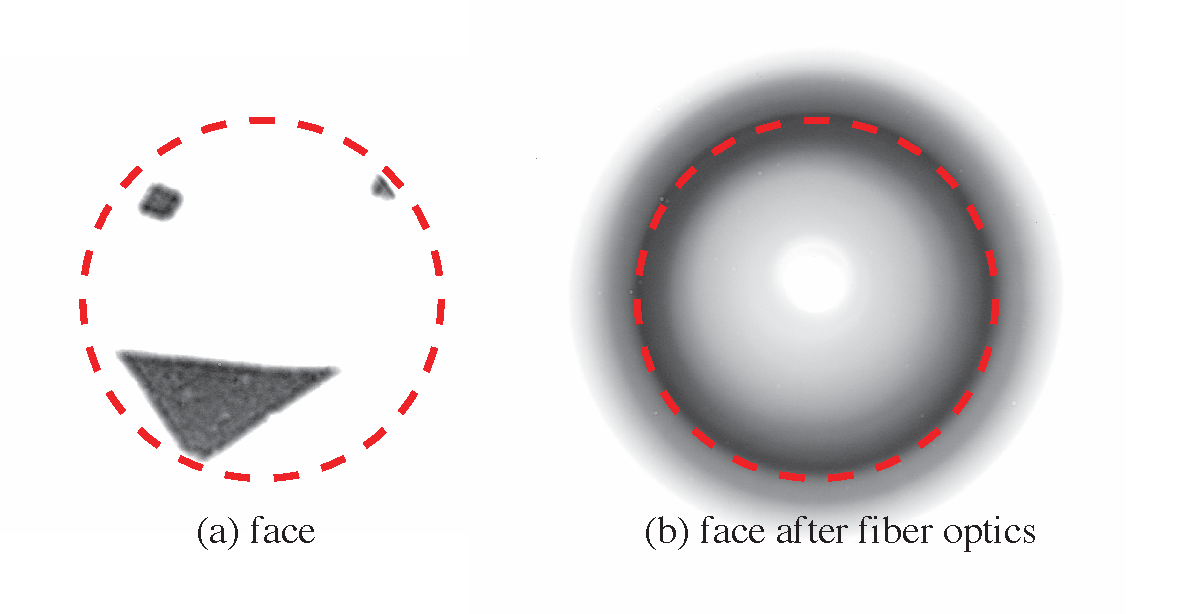
\includegraphics[width=\textwidth]{Introduction/figs/FRDude.pdf}
  \caption[Face on FRD]{\fixspacing\label{intro:fig:FRDude}The effects
    of fiber optics on an input signal. The face in (a) is smeared
    azimuthally and radially during its journey through an optical
    fiber. The red circle corresponds to the same angle at the
    input/output of the fiber.}
\end{figure}

With great power comes great responsibility, however, and fiber optics
affect the light passing through them in ways that have profound
implications for data quality and instrument design. In particular,
fiber optics not only attenuate precious astronomical light, but also
increase the entropy in the beam. The latter effect is referred to as
focal ratio degradation (FRD), whereby light injected into a fiber at
a particular angle emerges from the fiber at a larger angle. An
example of this is seen in Figure \ref{intro:fig:FRDude}; the light
coming out of the fiber (b) has been smeared to angles outside of the
maximum input angle (red circle). This increase in entropy creates a
need for larger (and more expensive) spectrograph optics and can
decrease the total system throughput if not properly accounted for. An
understanding of the causes of FRD can help mitigate its effects and
the first theories placed the blame on microbends along the length of
the fiber \citep{Gloge72,Carrasco94}. Recent studies have suggested
however, that most FRD is caused by scattering at the surface of the
fiber \citep{Avila98,Haynes11,Eigenbrot12}. In the latter scenario it
is likely that surface treatments (i.e., anti-reflective coatings) can
mitigate the effects of FRD.

\clearpage
\phantomsection % Fixes references link in hyperref/PDF index

% Requires thesis.bst to be present (or linked) in chapter subdirectory.
\bibliographystyle{thesis}
\bibliography{Introduction}

\chapter[Fiber Focal Ration Degradation]{The Angular and Wavelength Dependence of Fiber Focal Ratio Degradation}
\label{chap:FRD}

% Leave space between title and quote or publication note.  This has often been
% 10cm for a quote and 8 cm for a reference, but this is really up to you.
%\vspace{8cm}

%%%%%%%%%%%%%%%%%%%%%%%%%%%%%%%%%%%%%%%%%%%%%%%%%%%%%%%%%%%%% 
%% \begin{chabstract}
%%     Chapter abstract.
%% \end{chabstract}
%% \cleardoublepage

\section{Outline}
This is the work I did during my first two years. It was published in an SPIE
conference proceedings and is thus already done.

\section{Schedule}
This will take a maximum of 1 day to get all the formatting correct. No new
work has been done since the publication of the proceedings so it's pretty
much a drop in job.

\bibliographystyle{thesis}
\bibliography{FRD}

\chapter[\GP Construction]{\GP and HexPak: A Variable-pitch, Dual-head IFU for the WIYN 3.5m Bench Spectrograph}
\label{chap:pak_build}

% Leave space between title and quote or publication note.  This has often been
% 10cm for a quote and 8 cm for a reference, but this is really up to you.
%\vspace{8cm}

%%%%%%%%%%%%%%%%%%%%%%%%%%%%%%%%%%%%%%%%%%%%%%%%%%%%%%%%%%%%% 
%% \begin{chabstract}
%%     Chapter abstract.
%% \end{chabstract}
%% \cleardoublepage

\section{Outline}
We built some siiiick IFUs that one time. Let's talk about how we did it. This
\emph{could} just be a more-or-less drop in of Wood et al 2012, although I'm
not sure how legit that is. The other option is to not include this as a
chapter explicately and instead just reference the Wood paper in Chapter
\ref{chap:gradpak_obs}.

\section{Schedule}
Either this is copied from Wood et. al 2012 or doesn't exist. Either way I
don't see it taking more than 1 day.

\bibliographystyle{thesis}
\bibliography{pak_build}

\chapter[Using \GP]{Observing NGC 891 with \GP: Novel Observational and Data Reduction Techniques}
\label{chap:gradpak_obs}

% Leave space between title and quote or publication note.  This has often been
% 10cm for a quote and 8 cm for a reference, but this is really up to you.
%\vspace{8cm}

%%%%%%%%%%%%%%%%%%%%%%%%%%%%%%%%%%%%%%%%%%%%%%%%%%%%%%%%%%%%% 
%% \begin{chabstract}
%%     Chapter abstract.
%% \end{chabstract}
%% \cleardoublepage

\section{Outline}
Using \GP presented its own unique set of challenges. In this chapter I will
detail the observation and reduction techniques I developed to get useful data
from this new IFU.

One question I have is where to put my GradPak\_guide. Much of the information
in that document will be reused in this chapter, but some of the lower-level
items (e.g. program API) seem out of place in a thesis. The whole guide will
live online somewhere and maybe the lower-level stuff can go in an appendix or
something, but I'm not so sure.

This chapter will also detail the observing program that resulted in our set
of NGC 891 data. Things like observing logs, pointings, etc. will go here. As
the end product of both the new reduction techniques and the NGC 891 program
we will show some reduced spectra and make some broad scientific
interpretations.

\section{Schedule}
Much of this writing is already done. More importantly, all of the
developement/analysis is complete. I estimate a week of focused effort is more
than enough to finish this chapter.

\bibliographystyle{thesis}
\bibliography{GradPak_obs}

\chapter[Stellar Populations in NGC 891]{The Location of Stellar Populations in NGC 891}
\label{chap:891_pop}

% Leave space between title and quote or publication note.  This has often been
% 10cm for a quote and 8 cm for a reference, but this is really up to you.
%\vspace{8cm}

%%%%%%%%%%%%%%%%%%%%%%%%%%%%%%%%%%%%%%%%%%%%%%%%%%%%%%%%%%%%% 
%% \begin{chabstract}
%%     Chapter abstract.
%% \end{chabstract}
%% \cleardoublepage

\section{Outline}
Kind of the ``meat'' of the thesis. Here we go in depth about the analysis
methods used on the data described in \ref{chap:gradpak_obs}. The punchline is
some statement about how age (and, to a lesser precision, metallicty) varies
with radius and height in NGC 891.

\section{Basic Analysis}
\begin{itemize}
  \item Velocities
  \item Emission Correction
  \item Extinction Model
\end{itemize}
\subsection{Schedule}
This is basically done. The two things that still need work are 1) deciding
where exactly the extinction model section goes, and 2) basic editing. This
could be completed in 2 days.

\section{LOS Depths}
\begin{itemize}
  \item Velocity-based measurement
  \item Optical depth based measurement
\end{itemize}
\subsection{Schedule}
Great progress has been made over the last few days on this front. I think the
velocity stuff is done and 80\% written up.

The optical-depth section of this has a completed framework, but the analysis
depends on a lot of assumptions about the dust distribution that we will take
from other sources. This requires more thought. Still, a week should be
sufficient to complete this section.

\section{SSP Fitting}
\begin{itemize}
  \item Basic model
  \item Chisq weights
  \item Model Libraries
  \item Determining Age/Metallicity
\end{itemize}
\subsection{Schedule}
The first three bullet points above are basically done and need only basic
copy editing. This could be done in a few days.

The last bullet point is where we have been spending most of our time recently
and I think we are extremely close to being ``done'' with the actual
analysis. I mean, shit, we could say ``we're going to use weights because they
exclude known bad metallicities, and we're going to use this power because
we've sampled a coarse grid of powers and it does the best in terms of
rejecting metallicities, but not too many metallicities'' tomorrow and be done
with this. The pipline to produce ages and metallicities already exists, we're
just iterating on the uncertainties.

Once the anlysis is done this will take a week to write up.

\section{Spectral Indices}
\begin{itemize}
  \item Measurement
  \item Use as independent check on metallicities used in SSP fitting
  \item Qualitative results of trends in age, metallicity with height
\end{itemize}
\subsection{Schedule}
Some of this is already done. The last bullet point needs the most work. In
particular I have not settled on exactly what plane of spectral indices are
the most informative. Trager and Co. like Balmer vs <MgFe> and Balmer vs <Fe>,
but the latter of those does not work well with our galaxy models (dynamic
range is very small). We currently use \Hd vs <MgFe> and \Hd vs Mgb, but the
justification is lacking.

I think if we stay relatively shallow on this topic we can get everything
figured out relatively quickly. Maybe 1-2 weeks.

\section{Heating Models}
\begin{itemize}
  \item Model recipe
  \item comparison to data
\end{itemize}
\subsection{Schedule}
The ball is mostly in your court on this one. We have ages as a function of r
and z, now we need models for comparison. In principle this could be a very
short, ``look, we're not crazy'' section with an eye towards future, in depth
work.

\bibliographystyle{thesis}
\bibliography{891_pop}

\chapter[Doppler Tomography]{Decoding 3D Disk Struction and Dynamics Using Doppler Tomography}
\label{chap:SALT}

% Leave space between title and quote or publication note.  This has often been
% 10cm for a quote and 8 cm for a reference, but this is really up to you.
%\vspace{8cm}

%%%%%%%%%%%%%%%%%%%%%%%%%%%%%%%%%%%%%%%%%%%%%%%%%%%%%%%%%%%%% 
%% \begin{chabstract}
%%     Chapter abstract.
%% \end{chabstract}
%% \cleardoublepage

\section{Outline}
Hey, remember all the fun with SALT data? I sure do. We got pretty damn close
to having something cool a few times. I think the most concise and impactful
realization of this analysis was the stuff I present at Galaxies in 3D across
the Universe in Vienna, 2014.

\section{Schedule}
This is pretty tricky. If we want to persue any new analysis the potential for
lots of work becomes very high. I estimate that even just pulling together all
the basic information from various posters/proceedings/paper drafts into a
coherent chapter will take a week.

\bibliographystyle{thesis}
\bibliography{SALT}

\chapter[Conclusion]{Conclusion}
\label{chap:conclusion}

% Leave space between title and quote or publication note.  This has often been
% 10cm for a quote and 8 cm for a reference, but this is really up to you.
%\vspace{8cm}

%\vfil\eject\clearpage
\clearpage
NGC 891 offers a unique opportunity to perform stellar poulation
analyis and compare the results to our detailed understanding of the
distribution of stars in the Milky Way. In this way it occupies an
important bridge between the Milky Way and surveys that offer a large
sample size, but a smaller spatial resolution. The closeness and
nearly totally edge-on nature of NGC 891 also allows for unambiguous
determination of finely sampled vertical gradients in stellar
population, which makes it a perfect test-case for theories concerning
the origin of disk stratification seen in the Milky Way.

To take advantage of the information available in NGC 891 I helped
design and construct HexPak/\GP, a pair of fiber IFUs for the WIYN
telescope. In Chapter \ref{chap:pak_build} I detail the design and
fabrication of these instruments. The important features of HexPak/\GP
are:
\begin{enumerate}
\item HexPak has a standard hexagon shape made mostly of fibers with
  an on-sky diameter of 2\farcs8. It also has a high resolution core
  of 18 0\farcs94 fibers that make it idealy suited for studies of
  face-on galaxies or any bright object where high spatial resolution
  is desired.

\item \GP is roughly rectangular in shape and has five different fiber
  sizes ranging from 1\farcs87 - 5\farcs62. The regions of different
  size are arranged in a gradient that is optimized for to measure
  roughly expoentially decreasing surface brightness at roughly
  \val{10}{Mpc}; a similar S/N per fiber can be achieved in a single
  exposure. \GP is ideally suited for observations of objects with a
  large dynamic range in brightness where spectral resolution can be
  sacrificed for observing efficiency.

\item At the spectrograph input the slits of HexPak and \GP share a
  foot and focal plane. This allows observers to swap between the two
  IFUs with zero modifications to the Bench Spectrograph.

\item The head fixtures of HexPak and \GP, while physically separate,
  share a common focal plane in the WIYN IAS. This further eases the
  transition between the two IFUs. In practice an observer can switch
  between HexPak and \GP during an observing run in roughly 10
  minutes.

\end{enumerate}

During the conception and construction of HexPak/\GP I researched ways
to improve the optical performance of fiber-based instruments, mainly
through the mitigation of FRD. In Chapter \ref{chap:FRD} I detail my
experiements, which are broadly applicable to all fiber optic systems,
and find:
\begin{enumerate}

\item FRD is dominated by light entering the fiber at smaller angles
  (i.e., closer to the axis of light propogation).

\item A secondary component of FRD is attributable to the end-polish
  of fiber surfaces. FRD decreases with polishing down to finer grit
  sizes, but not significantly below grit-sizes of 5\mum.

\item Total throughput also depends on end-polish, with a wavelength
  dependence that indicates the increase in throughput is simply a
  reduction in surface-scattering.  The most significant gains occur
  for polishing that proceeds down to 5 $\mu$m grit, although for most
  astronomical applications at low light-levels polishing finer than
  this level is measurably advantageous.

\item The amount of FRD does \textbf{not} depend on wavelength.

\end{enumerate}

Chapter \ref{chap:891_1} details the first set of results from a
program that measures stellar populations in NGC 891 with \GP. In this
chapter I detail challenges in data acquisition/reduction caused by
the unique nature of \GP, but also present methods that largely
eliminate any negative impact on the resulting data.

I also describe the observing program that is designed to cover NGC
891 out to large heights and radii. The design of \GP is ideally
suited to a program of this nature and allows for efficient collection
of high-quality data.

I then use the well known and characterized LICK spectral index system
to identify separate stellar populations in NGC 891 and find:
\begin{enumerate}

\item There is a clear transition with height above NGC 891's disk
  midplane between young and old populations at \val{0.4}{kpc}
  (roughly the broad-band exponential scale-height). This is
  consistent with models of heating of the stellar disk in the solar
  cylinder.

  \item For $|z| > \val{0.4}{kpc}$ there is a trend towards younger
    populations at larger projected radii, consistent with an
    inside-out formation history in NGC 891. The trend also suggests a
    flaring of the young stellar disk at radii beyond 8 kpc.

  \item Beyond 8 kpc in radius and between 0.4 kpc $\leq |z| <$ 1 kpc
    there is a a clear asymmetry in age between the two sides of the
    galaxy. The approaching side, where there is more H$\alpha$
    emission, appears younger. This can be explained by spiral
    structure in NGC 891; on the approaching side of the galaxy we see
    the leading edge of a spiral arm that has very recent/ongoing star
    formation. Our sight-lines to the receeding side of the galaxy,
    however, look onto the trailing edge of another arm that is
    obscured by high concentrations of dust.

\end{enumerate}

Finally, in Chapter \ref{chap:891_2} I employ the power of
full-spectrum fitting to get a detailed and quantitaive view of
stellar populations in NGC 891. To confidently interpret the results
of this method I need to understand the interplay between all of the
fit parameters, namely the well known degeneracies between age,
metallicity, and extinction. Furthermore, assumptions about the star
formation history in NGC 891 can introduce large systematics in our
results.

The degeneracies between age, metallicity, and extinction are
exacerbated by SSP template libraries that constitute a large set of
individual SSPs with little thought to the astrophysical similarities
that exist over a wide range of age and metallicity values. In other
words, most SSP template libraries have many SSPs that, while assigned
different age or metallicity values, have very similar spectra. To
mitigate these degeneracies I use diffusion k-means to create a new
SSP basis set that greatly reduces the number of SSP templates while
still preserving important astrophysical features. With this new SSP
basis set I estimate the uncertainty in fit parameters caused by
degeneracies between the model spectra to be roughly 10\% for age and
extinction and \asim 20\% for metallicity.

I also quantify the systematic age uncertainty that arises from
assuming a star formation history during the interpretation of the
fitting results. In the worst case these uncertainties are \asim 20\%,
but I argue that the worst case (totally random star formation on
small physical scales) is unrealistically pessimistic for our
data. NGC 891 is a coherent galaxy and over long timescales (\asim 1
Gyr) the star formation history should be relatively the same across
the entire galaxy. Thus the systematic uncertainties do not apply when
comparing detailed structure within NGC 891; they are only important
when comparing NGC 891 to other galaxies that may have different star
formation histories.

With an understanding of uncertainties in my results I identify three
features in NGC 891 that are distinct from one another in a position,
age, metallicity, extinction phase space. They are:
\begin{enumerate}

\item A ``primary'' disk that exists at all heights and radii less
  than \val{8}{kpc}. In this disk there is clear evidence for the
  presence of young stellar populations ($< \val{\asim 400}{Myr}$ ago)
  below \val{0.4}{kpc} and a lack of the same populations above
  \val{0.4}{kpc}, consistent with the results of Chapter
  \ref{chap:891_1}. Above this transition emission from the disk is
  dominated by intermediate and old stars and the average population
  age increases with height. This disk also exhibits negative
  metallicity gradients with both radius and height, which is
  consistent with observations of the Milky Way. It is also likely
  that the primary ``disk'' is actually a superposition of multiple
  disk components previously identified in NGC 891.

\item A flared extension of the the primary disk at radii beyond
  \val{8}{kpc}. This flare has the same age and metallicity properties
  as the main disk, but with a scale height roughly twice as
  large. This increase in scale height decreases the total surface
  density of dust at large radii and the extinction is correspondingly
  lower, especially near the midplane.
  
\item A sequence of intermediate-age, super-solar metallicity
  populations at large heights ($|z|> \val{\asim 0.9}{kpc}$) and radii
  ($r>\val{8}{kpc}$). Despite their old ages, the populations in this
  ``third sequence'' appear to come from a fundamentally different
  underlying distribution compared to stars at similar heights but
  smaller radii. Despite an overall higher metallicity this third
  sequence still shows internal metallicity gradients in $r$, and $z$
  consistent with the trends seen in the primary disk and flare. The
  origin of this population is not easily explained and any theories
  about it will need to contend with its curious combination of old
  ages and high metallicities that occur far from the center of the
  galaxy.

\end{enumerate}

This work constitutes one of the first detailed, resolved studies of
stellar populations in a nearby galaxy and as such lays the groundwork
for future studies. In particular, the methods outlined here could
easily be applied to other nearby, edge-on galaxies. This thesis
provides a robust set of tools, from instruments to data reduction and
analysis methods, that will allow future astronomers to rapidly expand
our view of stellar populations and disk formation.

\clearpage
\phantomsection % Fixes references link in hyperref/PDF index

% Requires thesis.bst to be present (or linked) in chapter subdirectory.
\bibliographystyle{thesis}
\bibliography{Introduction}


% See the thesis.cls file for the steps to convert AASTeX papers
% into thesis chapters

%%%%% ADD APPENDICES %%%%%%%%%%%%%%%%%%%%%%%%%%%%%%%%%%%%%%%%%%%%%%%%%%%%%%%%%%%

%\addtocontents{toc}{\protect\vspace{0.5cm}}
                        % Add some vertical space to the table of contents
                        %   file before listing the appendices (the \protect
                        %   command is necessary because \vspace is fragile).

%\appendix		% Resets chapter numbering to A, B, C... for appendices

%\include{apA}		% *.tex file for Appendix A (just like a chapter)

%\include{vitae}         % *.tex file for the Vitae

%\include{colophon}      % *.tex file for the Colophon

% END THE DOCUMENT %%%%%%%%%%%%%%%%%%%%%%%%%%%%%%%%%%%%%%%%%%%%%%%%%%%%%%%%%%%%%

%\clearpage
%Need to uncomment all of the following to get an index
%\addcontentsline{toc}{section}{Index}
%{\fixspacing \small
%\printindex
%}

\end{document}
